%%%%%%%%%%%%%%%%%%don't forget if needed %%%%%%%%%%%%%%%%%%%%%
%\section[toc version]{title version%
%              \sectionmark{head version}}
%\sectionmark{head version}
%%%%%%%%%%%%%%%%%%%%%%%%%%%%%%%%%%%%%%%%%%%%%%%%%%%%%%%%%%%%%%
\def\titcourt{Numerical simulation of 3D configurations using domain decomposition method}
\def\titlong{Numerical simulation of 3D configurations using domain decomposition method}
%%%%%%%%%%%%%%%%%%%%%%%%%%%%%%%%%%%%%%%%%%%%%%%%%%%%%%%%%%%%%%%%
\chapter[\titlong]{\titlong%
              \chaptermark{\titcourt}}
\chaptermark{\titcourt}
\label{chap-3D-SIMULATION}
%%%%%%%%%%%%%%%%%%%%%%%%%%%%%%%%%%%%%%%%%%%%%%%%%%%%%%%%%%%%%%%%
%%%%%%%%%%%%%%%%%%%%%%%%%%%%%%%%%%%%%%%%%%%%%%%%%%%%%%%%%%%%%%%%

Having extensively validated and analysed 2D  melting and solidification configurations for phase-change materials in the previous chapters, we now perform parallel computing of three-dimensional liquid-solid phase-change systems involving natural convection.
We use the recent library \texttt{ffddm} that makes available in FreeFem++ state-of-the-art scalable Schwarz domain decomposition methods (DDM).
Our motivation to expand our numerical model to 3D configuration is first motivated by the lack of publications in the literature for accurate 3D simulations of phase-change materials.
%Also, since publications related to three-dimensional simulation of phase-change material is not abundant in the literature, we expand our numerical model to 3D configuration.
Also, experimental investigations against which we have validated our numerical method involve three-dimensional effects that we have assumed to be neglected in our comparisons.
The later assumption is however no more valid for high $\Ray$ numbers.

The main feature of our numerical approach is the use of 3D adaptive mesh, performed using \textit{mmg3d} library.
\textit{Mmg3d} is a 3D remeshing software developed by \cite{dobrzynski:hal-00681813}, which allows to remesh an initial mesh made of tetrahedra.
The metrics for the mesh adaptation are computed using \textit{mshmet} library, which computes anisotropic metric based on solution variations. 
We use \textit{Metis} library to split the domain into subdomains.
For three-dimensional applications, direct solvers used in the frame of 2D problems are not appropriate and iterative methods must be employed since memory requirements for \textit{LU} decomposition would rapidly exceed the capacity of available computers.
The linear system of equations resulting from the Newton linearisation are thus solved using \textit{GMRES} Krylov method.
Since it is well known that iterative methods can suffer from convergence problems, we adapt the number of subdomain with the number of d.o.f. in such a way that each processor could handle $1,000$ tetrahedra.
The Optimized Restricted Additive Schwarz (ORAS) preconditioned \textit{GMRES} solver proved to be extremely efficient since an order of 30 iterations were necessary to get a residual norm of $10^{-9}$ for each Newton iteration.
We note that in all numerical simulations, a quadratic ($\PP_2$) discretization of $\theta$ was used.

The remainder of this chapter is as follows.
In Sec. \ref{sec: natconv-air-3D}, we validate the 3D natural convection of air in differentially heated cube against numerical results by \cite{Wakashima-2004}.
We compare moreover the solutions obtained by the parallel computation with the solution obtained using sequential algorithms.
The natural convection of air in a cube box including heated obstacle is also performed.
The natural convection of water is then presented in Sec. \ref{sec-3D-water-convec}.
Finally, the lateral melting of n-octadecane PCM inside 3D enclosure is considered.

%We solve the system of Eqs. \ref{eq-qmvt} - \ref{eq-energ} without the penalty term $A(\theta) \vec u$ in the momentum equation and the source term $\partial (CS)/\partial t$ in the energy equation.
%Linear and non-linear expressions of the buoyancy force $f_B(T)$ in the Boussinesq approximation (\ref{eq-energie-enth-model}) are investigated, by simulating the natural convection of air and the natural convection of water.
%Natural convection of water exhibits actually a non-linear variation of the density with a maximum value around $T=4^o C$ while linear variation is generally assumed for the natural convection of air in the Boussinesq approximation.

\section{Numerical simulation of the natural convection of air in 3D configurations}\label{sec: natconv-air-3D}
 Following the same line of argument that was outlined in Chapters. \ref{chap-NATCONV} and \ref{chap-MELTING}, we start by presenting the natural convection of air, that involves linear description of the buoyancy force $f_B$, and include gradually additional non-linearities.
The well-known thermally driven cavity is addressed first in Sec. \ref{subsec-3D-natconv-air} and the problem is then complicated by incorporating heated cube in the center of the domain in Sec. \ref{sub-OBSTACLE-3D}.
The physical parameters are the same than used in the 2D simulations ($\Prd = 0.71$) and we investigate three Rayleigh numbers: $\Ray=10^4$, $\Ray=10^5$, and $\Ray=10^6$. 
The walls are rigid and impermeable. The vertical walls at $x=0$ and $x=1$ are isothermal and have different temperatures $T_h=0.5$ and $T_c=-0.5$ respectively. The remaining walls are considered adiabatic. 
The fluid is initially at rest and the temperature is linearly distributed from the cold to the hot walls.
We solve only the steady Eq. \ref{eq-weak-steady} by increasing smoothly the parameter $\alpha$ before the Boussinesq term (which can be assimilated to a Rayleigh continuation step) with a maximum of $6$ steps for $\Ray = 10^6$.

\subsection{Natural convection of air in differentially heated cube box} \label{subsec-3D-natconv-air}

\begin{table}[!ht]
	\begin{center}
		\begin{tabular}{|*{6}{c|}}
			\hline
			 $\Ray$ & \em{nb proc }                  & $||u||_{2}$                        & $||u||_{\infty}$                & $||T||_{2}$              & $||T||_{\infty}$\\ \hline \hline
			\multirow{4}{*}{$10^4$} & 28 & $1.12496 \cdot 10^{-6}$ & $3.1 \cdot 10^{-6}$ & $ 3.09966 \cdot 10^{-6} $ & $7 \cdot 10^{-6}$ \\% \hline
			\cline{2-6}
			& 42 & $1.53698 \cdot 10^{-6}$ & $5.1 \cdot 10^{-6}$ & $ 3.23352 \cdot 10^{-6} $ & $8 \cdot 10^{-6}$ \\ \cline{2-6} %\hline 
			& 56 & $1.55576 \cdot 10^{-6}$ & $5.1 \cdot 10^{-6}$ & $ 3.4342 \cdot 10^{-6} $ & $8 \cdot 10^{-6}$  \\ \cline{2-6} %\hline
			& 70 & $1.25622 \cdot 10^{-6}$ & $3.6 \cdot 10^{-6}$ & $ 3.56048 \cdot 10^{-6} $ & $8 \cdot 10^{-6}$ \\ \hline \hline
			\multirow{4}{*}{$10^5$} & 28 & $1.73254 \cdot 10^{-6}$ & $6.1 \cdot 10^{-6}$ & $ 2.40467 \cdot 10^{-6} $ & $7 \cdot 10^{-6}$ \\% \hline
			\cline{2-6}
			& 42 & $2.84973 \cdot 10^{-6}$ & $7.78 \cdot 10^{-6}$ & $ 3.53003 \cdot 10^{-6} $ & $9 \cdot 10^{-6}$ \\ \cline{2-6} %\hline 
			& 56 & $3.00832 \cdot 10^{-6}$ & $7.39 \cdot 10^{-6}$ & $ 4.17769 \cdot 10^{-6} $ & $1.1 \cdot 10^{-5}$  \\ \cline{2-6} %\hline
			& 70 & $3.68118 \cdot 10^{-6}$ & $9 \cdot 10^{-6}$ & $ 4.70846 \cdot 10^{-6} $ & $1.2 \cdot 10^{-5}$ \\ \hline \hline
			\multirow{4}{*}{$10^6$} & 28 & $6.61804 \cdot 10^{-6}$ & $1.826 \cdot 10^{-5}$ & $ 3.46504\cdot 10^{-6} $ & $1.1 \cdot 10^{-5}$ \\% \hline
			\cline{2-6}
			& 42 & $5.93966 \cdot 10^{-6}$ & $1.5 \cdot 10^{-5}$ & $ 3.98082 \cdot 10^{-6} $ & $1.2 \cdot 10^{-5}$ \\ \cline{2-6} %\hline 
			& 56 & $7.05144 \cdot 10^{-6}$ & $1.9247 \cdot 10^{-5}$ & $ 5.0044 \cdot 10^{-6} $ & $2 \cdot 10^{-5}$  \\ \cline{2-6} %\hline
			& 70 & $6.02152 \cdot 10^{-6}$ & $1.68 \cdot 10^{-5}$ & $ 4.50094 \cdot 10^{-6} $ & $1.8 \cdot 10^{-5}$ \\ \hline
		\end{tabular}
	\end{center}
	\caption {3D differentially heated cavity. Comparison between sequential and ffddm algorithm for uniform grids of $40 \times 40 \times 40$ }
	\label{tab-T1}
\end{table}

We first compare the current simulation with the numerical data of \cite{Wakashima-2004}, who have used a forth order finite difference method, with a vorticity-stream function formulation with different uniform meshes of  $120 \times 120 \times 120 \times 10$ grid nodes.
Our results were obtained using uniform grids of $ 40 \times 40 \times 40$.
Since the converged flow pattern and temperature distributions are symmetrical with respect to the center of the cavity for the investigated Rayleigh number,
we display in 
Fig. \ref{fig-3DT} the temperature field at the mid section ($y = 0.5$), for each of the three Rayleigh numbers $\Ray = 10^4$ (top), $\Ray = 10^5$ (middle), $\Ray = 10^6$(bottom).  
On the left we display the numerical results of \cite{Wakashima-2004} and on the right the present simulation.
The comparison with the benchmark solution exhibits a fairly good agreement with the considered test case.
The higher the Rayleigh number, the thinner the thermal boundary layer thickness in the vicinity of the vertical walls.
One can also notice the stagnant fluid with stratified temperature in the center of the domain in both numerical solutions.



The parallel solver is moreover compared with the sequential algorithm to assess the consistency of our method with the number of subdomains.
We compute $L^2$ and $L^\infty$ norms of the velocity and the temperature and report the result in Tab. \ref{tab-T1} for all cases.
The difference between both algorithm is of order of $10^{-6}$.
and we do not observe a large variation of the error when the number of subdomains keep increasing.
The number of subdomain varies from $28$ to $70$ for $1.8$ millions of unknown.
The comparison with the sequential algorithm was limited to $40 \times 40 \times 40$ grids size since the simulations are highly demanding in CPU time.
The steady state solution required $57$ CPU hours and $3$ runs (restarts) with $120$ Go of memory for the sequential algorithm, for the highest value of the Rayleigh number. 
The computational time is considerably reduced and 3D simulations becomes affordable by using DDM since only $21$ CPU minutes  ($1308.48$ s) were necessary with $70$ processors to achieve the same case with an error of $6.02152 \cdot 10^{-6}$ on $\vec u$ and $ 4.50094 \cdot 10^{-6} $ on $\theta$.

When compared to the two-dimensional case, the flow inside the 3D cubic box is obviously more complex.
Indeed, a spiral movement of the fluid along the walls is observed whereas boundary layer heat transfer takes place in the same region.

\begin{figure}[!ht]
\begin{minipage}{\linewidth}
\begin{center}
 {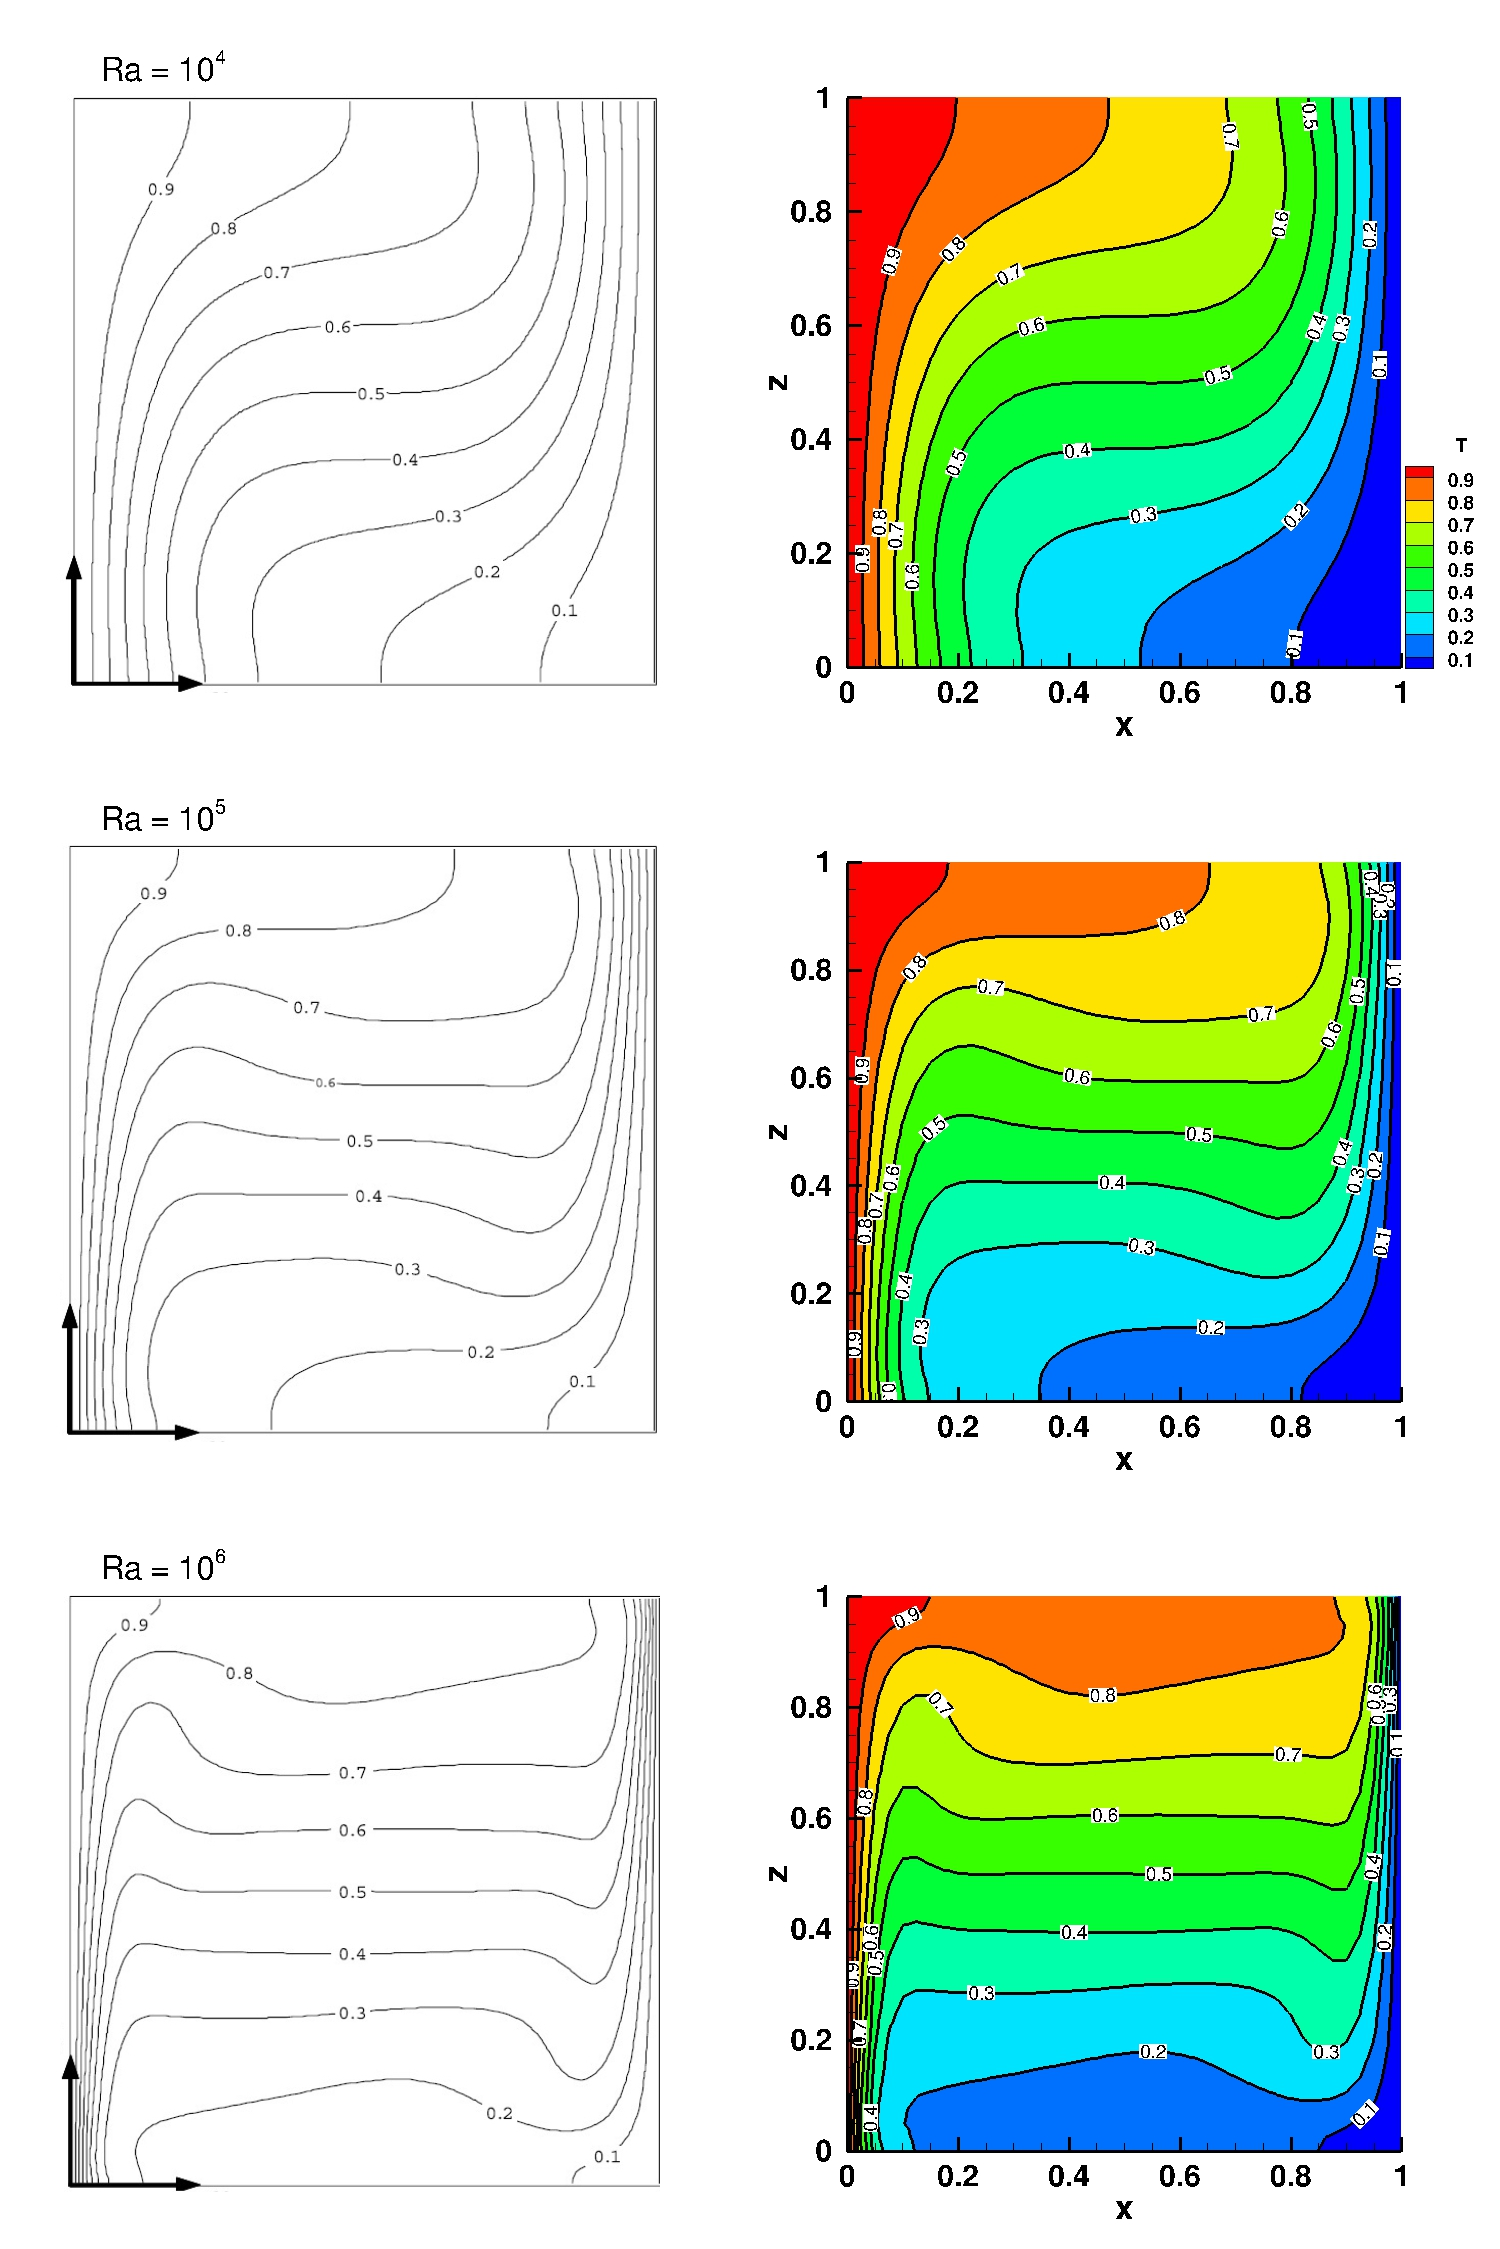
\includegraphics[width=.95\textwidth]{\figpath/Fig_cap_natconv/Validation_3D_seq_T1}}
\end{center}
\end{minipage}
\caption{3D differentially heated cavity. Temperature contours at the mid-plane of ($y=0.5$); comparison with the results of \cite{Wakashima-2004} (left images). }
\label{fig-3DT} 
\end{figure}

\subsection{Natural convection in a cube with an inner heated obstacle}\label{sub-OBSTACLE-3D}
A heated obstacle is then included in the center of the unit cube as depicted in Fig. \ref{fig-obstacle-Ra1e4}.


\begin{table} [!ht]
	\begin{center}
		\begin{tabular}{|*{7}{c|}}
			\hline
			 $\Ray$ & \em{nbseg} & \em{nb proc }                    & $||u||_{2}$                        & $||u||_{\infty}$                & $||T||_{2}$              & $||T||_{\infty}$\\ \hline \hline
%			\multirow{12}{*}{$10^4$} & \multirow{4}{*}{40} & 28 & $0.00087137$ & $0.0058298$ & $ 0.0022491 $ & $0.01592$ \\
%			\cline{3-7}
%			& & 42 & $0.000870796$ & $0.0058292$ & $ 0.00224866 $ & $0.015921$ \\ \cline{3-7} %\hline 
%			& & 56 & $0.000870646$ & $0.0058293$ & $ 0.00224788 $ & $0.015921$  \\ \cline{3-7} %\hline
%			& & 70 & $0.000870747$ & $0.0058286$ & $ 0.00224795 $ & $0.015921$ \\ \cline{2-7}
%			 & \multirow{4}{*}{60} & 112 & $0.000785593$ & $0.0021$ & $ 0.000858912 $ & $0.010024$ \\% \hline
%			\cline{3-7}
%			& & 140 & $0.000783164$ & $0.002097$ & $ 0.000865668 $ & $0.010024$ \\ \cline{3-7} %\hline 
%			& & 168 & $0.000779419$ & $0.002091$ & $ 0.000858384 $ & $0.010027$  \\ \cline{3-7} %\hline
%			& & 196 & $0.000767662$ & $0.00209$ & $ 0.000864693 $ & $0.010019$ \\ \cline{2-7}
%			 & \multirow{4}{*}{80} & 224 & $0.000637268$ & $0.001795$ & $ 0.000551538 $ & $0.001661$ \\% \hline
%			\cline{3-7}
%			& & 238 & $0.000152936$ & $0.000548$ & $ 0.000205031 $ & $0.000634$ \\ \cline{3-7} %\hline 
%			& & 252 & $0.000239786$ & $0.000841$ & $ 0.000231648 $ & $0.000661$  \\ \cline{3-7} %\hline
%			& & 266 & $0$ & $0$ & $ 0 $ & $0$ \\ \hline 
			\multirow{12}{*}{$10^6$}& \multirow{4}{*}{40} & 28 & $0.0011359$ & $0.0089746$ & $ 0.00401922 $ & $0.020067$ \\% \hline
			\cline{3-7}
			& & 42 & $0.00113742$ & $0.0089788$ & $ 0.00402103 $ & $0.020067$  \\ \cline{3-7} %\hline 
			& & 56 & $0.00113625$ & $0.0089768$ & $ 0.00402081 $ & $0.020063$   \\ \cline{3-7}%\hline
			& & 70 & $0.0011348$ & $0.0089726$ & $ 0.00401999 $ & $0.020065$  \\ \cline{2-7} %\hline
			 & \multirow{4}{*}{60} & 112 & $0.000765582$ & $0.0022345$ & $ 0.00166687 $ & $0.015296$ \\% \hline
			\cline{3-7}
			& & 140 & $0.000763449$ & $0.0022313$ & $ 0.00166143 $ & $0.015257$ \\ \cline{3-7} %\hline 
			& & 168 & $0.000763074$ & $0.0022176$ & $ 0.00166605 $ & $0.015284$  \\ \cline{3-7} %\hline
			& & 196 & $0.000760368$ & $0.0022093$ & $ 0.00167368 $ & $0.015299$ \\ \cline{2-7} 
			 & \multirow{4}{*}{80} & 224 & $0.00051462$ & $0.0016627$ & $ 0.000574467 $ & $0.001794$ \\% \hline
			\cline{3-7}
			& & 238 & $5.17443 \times 10^{-05}$ & $0.0001934$ & $ 0.00018074 $ & $0.0005666$ \\ \cline{3-7} %\hline 
			& & 252 & $8.68245 \times 10^{-05}$ & $0.000319$ & $ 8.11788 \times 10^{-05} $ & $0.000335$  \\ \cline{3-7} %\hline
			& & 266 & $0$ & $0$ & $ 0 $ & $0$ \\ \hline 

		\end{tabular}
	\end{center}
	\caption {3D convection in a cube with an inner heated cube. Comparison between sequential and ffddm algorithm for uniform grids of $40 \times 40 \times 40$ for $Ra = 10^4$ and $80 \times 80 \times 80$ for $Ra = 10^5$}
	\label{tab-T2}
\end{table}






\begin{figure} [!ht]
\begin{center}
\begin{minipage}{\linewidth}
 {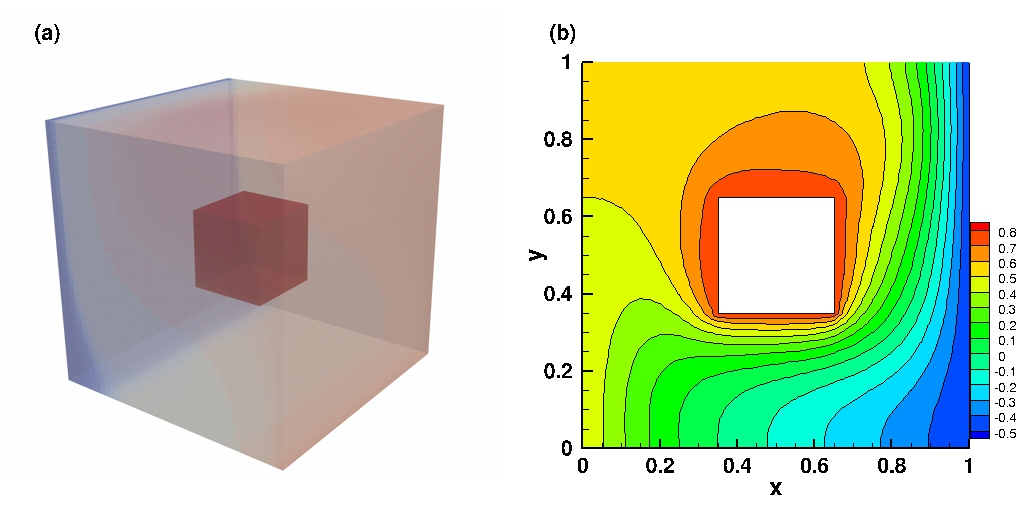
\includegraphics[width=0.98\textwidth]{\figpath/Fig_cap_natconv/3D_OBSTACLE_field}}
\end{minipage}
\end{center}
\caption{3D convection in a cube with an inner heated cube. Temperature fields for $Ra = 10^4$.}
\label{fig-obstacle-Ra1e4} 
\end{figure}

\clearpage
\newpage
\section{Numerical simulation of the natural convection of water in a cube cavity.} \label{sec-3D-water-convec}
